\begin{frame}[fragile]
\frametitle{Documento}
\framesubtitle{Ferramentas para trabalhos em linguística}

\begin{enumerate}
    \item caracteres IPA
    \item árvores sintáticas
    \item árvores de dependências
    \item exemplos enumerados
\end{enumerate}

\end{frame}

\begin{frame}[fragile]
\frametitle{Documento}
\framesubtitle{escrita fonética}
  \scriptsize
  \begin{columns}[c]
  \column{.5\textwidth}
  \begin{verbatim}
   \usepackage{tipa}
   
   \textipa{abcdefghijklmnopqrstuvwxyz}
   \textipa{ABCDEFGHIJKLMNOPQRSTUVWXYZ}
   \textipa{1234567890 @}
   \textipa{\:d \:l \:n \:r \:s \:t \:z}
   \textipa{\!b \!d \!g \!j \!G \!o}
  \end{verbatim}
  \column{.5\textwidth}
  \begin{fmpage}{\textwidth}
   \textipa{abcdefghijklmnopqrstuvwxyz}
   \textipa{ABCDEFGHIJKLMNOPQRSTUVWXYZ}
   \textipa{1234567890 @}
   \textipa{\:d \:l \:n \:r \:s \:t \:z}
   \textipa{\!b \!d \!g \!j \!G \!o}
  \end{fmpage}
  \end{columns}
  
  \url{https://www.tug.org/TUGboat/tb17-2/tb51rei.pdf}
  \url{https://ctan.org/pkg/tipa}
\end{frame}


\begin{frame}[fragile]
\frametitle{Documento}
\framesubtitle{tabela com códigos dos símbolos do IPA}
\vspace{-4ex}
\begin{figure}[h!]
  \centering
  \label{fig:tux}
  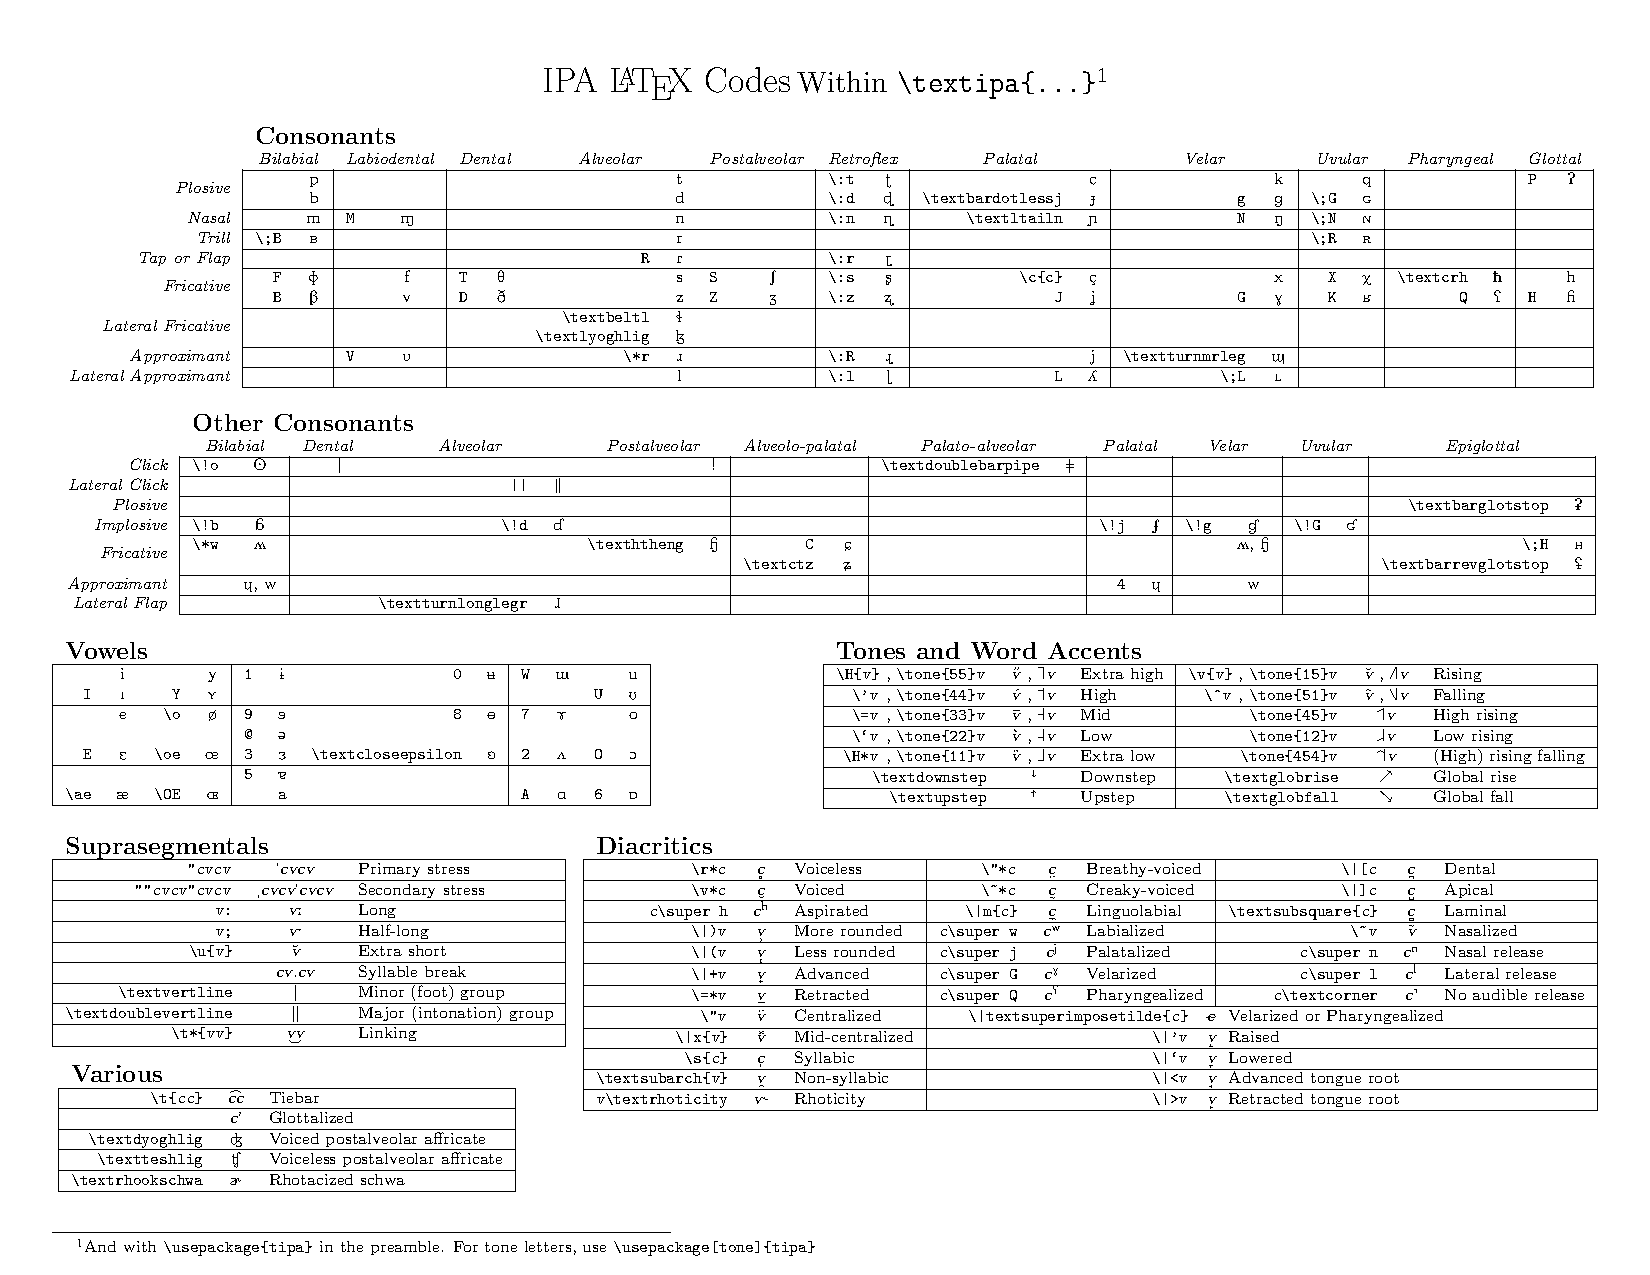
\includegraphics[width=\textwidth]
                     {figures/tipachart_mod.pdf}
  \caption{Tux.}
\end{figure}
\end{frame}



\begin{frame}[fragile]
\frametitle{Documento}
\framesubtitle{regras fonológicas}
  \scriptsize
  \begin{verbatim}
\usepackage{phonrule}
  
\phonb{\phonfeat{+stop \\ +consonant \\ +alveolar} }{[\textipa{R}]}
{\phonfeat{+vowel \\ +stressed} }{\phonfeat{+vowel \\ +stressed} }
  \end{verbatim}

  \begin{fmpage}{\textwidth}
\phonb{\phonfeat{+stop \\ +consonant \\ +alveolar} }{[\textipa{R}]}{\phonfeat{+vowel \\ +stressed} }{\phonfeat{+vowel \\ +stressed} }
  \end{fmpage}

\end{frame}


\begin{frame}[fragile]
\frametitle{Documento}
\framesubtitle{árvores sintáticas}
  \scriptsize
  \begin{columns}[c]
  \column{.5\textwidth}
  \begin{verbatim}
\begin{center}
\Tree [.S [.NP LaTeX ] [.VP [.V is ] 
  [.NP fun ] ] ]
\end{center}
  \end{verbatim}
  \column{.5\textwidth}
  \begin{fmpage}{\textwidth}
\begin{center}
\Tree [.S [.NP LaTeX ] [.VP [.V is ] [.NP fun ] ] ]
\end{center}
  \end{fmpage}
  \end{columns}
\end{frame}


\begin{frame}[fragile]
\frametitle{Documento}
\framesubtitle{Árvodre de dependência}
  \scriptsize
  \begin{verbatim}
   \usepackage{tikz-dependency}

    % In the document:
   \begin{dependency}[theme = simple]
   \begin{deptext}[column sep=1em]
      A \& hearing \& is \& scheduled \& on \& the \& issue \& today \& . \\
   \end{deptext}
   \deproot{3}{ROOT}
   \depedge{2}{1}{ATT}
   \depedge[edge start x offset=-6pt]{2}{5}{ATT}
   \depedge{3}{2}{SBJ}
   \depedge{3}{9}{PU}
   \depedge{3}{4}{VC}
   \depedge{4}{8}{TMP}
   \depedge{5}{7}{PC}
   \depedge[arc angle=50]{7}{6}{ATT}
   \end{dependency}
  \end{verbatim}
\end{frame}


\begin{frame}[fragile]
\frametitle{Documento}
\framesubtitle{Árvodre de dependência}
 
  \begin{fmpage}{\textwidth}
   \begin{dependency}[theme = simple]
   \begin{deptext}[column sep=1em]
      A \& hearing \& is \& scheduled \& on \& the \& issue \& today \& . \\
   \end{deptext}
   \deproot{3}{ROOT}
   \depedge{2}{1}{ATT}
   \depedge[edge start x offset=-6pt]{2}{5}{ATT}
   \depedge{3}{2}{SBJ}
   \depedge{3}{9}{PU}
   \depedge{3}{4}{VC}
   \depedge{4}{8}{TMP}
   \depedge{5}{7}{PC}
   \depedge[arc angle=50]{7}{6}{ATT}
   \end{dependency}
  \end{fmpage}

\end{frame}